 \documentclass{report}
 
\usepackage[utf8]{inputenc} 
\usepackage[T1]{fontenc}      
\usepackage[top=2.0cm, bottom=3cm, left=3.0cm, right=3.0cm]{geometry}
\usepackage{graphicx}
\usepackage{wrapfig}
\usepackage{amsmath,esint }
\usepackage{amssymb}
\graphicspath{{figures/}{../figures}}

\newcommand*\dif{\mathop{}\!\mathrm{d}}
\newcommand*\diver{\mathop{}\!\mathrm{div}}
\newcommand*\grad{\mathop{}\!\mathrm{grad}}

\begin{document}

\section*{Sillage d'un avion}

\begin{itemize}

	\item[$\circ$] On retrouve l'équation d'Alembert à partir de trois équation. Sur la masse volumique et la compressibilité :
	\begin{align*}
		\mu = \chi_sp\rho_0
	\end{align*}
	Sur l'équation de la conservation de la masse :
	\begin{align*}
		\frac{\partial \mu}{\partial t}+\grad(p)=0
	\end{align*}
	et l'équation d'Euler :
	\begin{equation}
		\rho_0\frac{\partial \vec{v}}{\partial t}+\vec{\grad}(\vec{v})=0
	\end{equation}
	On trouve alors une équation d'Alembert sur $\mu$, $\vec{v}$ et $p$, avec une célérité $c=1/\sqrt{\chi_s\rho_0}$

	\item[$\star$] Il faut raisonner en calculant l'écart entre 2 "bips" émis par l'avion à la période $T$. Soit $t_1=t$ et $t_2=t+T$ les temps où l'avion émet 2 bips à partir du temps $t$. Soient $t'_1$ et $t'_2$ les temps auxquels sont reçus les signaux par l'observateur. Comme l'onde se propage à la vitesse $c$ : $t'_1=t_1+d_1/c$ et $t'_2=t_2+d_2/c$ avec $d_1$ et $d_2$ les distances entre l'avion et l'observateur. La période entendue par l'observateur est :
	\begin{align*}
		T'=t'_2-t'_1=\frac{h}{c}\left(\frac{1}{\sin\theta(t_2)}-\frac{1}{\sin\theta(t_1)} \right) +T=-\frac{h\delta\theta\cos\theta(t_1)}{\sin^2\theta(t_1)} +T 
	\end{align*}
	En notant $\delta\theta=\theta(t_2)-\theta(t_1)\ll1$. Pour trouver $\delta\theta$ :
	\begin{align*}
		\tan\theta(t_2)-\tan\theta(t_2)=h\left(\frac{1}{x(t_1)}-\frac{1}{x(t_1)-vT} \right) =-\frac{vTh}{x(t_1)}=\frac{\delta\theta}{\cos^2\theta(t_1)}
	\end{align*}
	Donc $\delta\theta=-vT\sin^2\theta(t_1)/h$
	On trouve alors au final :
	\begin{align*}
		T'=T\left(1-\frac{v}{c}\cos\theta \right) 
	\end{align*}
	\item[$\star$] Les ondes émises sont sous forme de sphère, donc en théorie tout l'espace peut être atteint par le bruit de l'avion s'il vole depuis un temps infini. On entend l'avion avant qu'il passe devant l'observateur.

	\item[$\diamond$] L'onde émise à l'instant $t$ parcourt une distance $d(t)=\sqrt{x^2+h^2}$ avant d'arriver à l'observateur. Donc :
	\begin{align*}
		t'=t+\sqrt{\frac{h^2}{c^2}+\frac{v^2t^2}{c^2}}
	\end{align*}

Si $t\longrightarrow-\infty$, $t'\longrightarrow (1-v/c)t>0$ (attention à la valeur absolue dans le cas $t<0$ !). car $v>c$ et $t<0$. Si $t\longrightarrow+\infty$, $t'\longrightarrow (1+v/c)t>0$, avec une pente plus forte.

\begin{figure}[h!]
\centering
		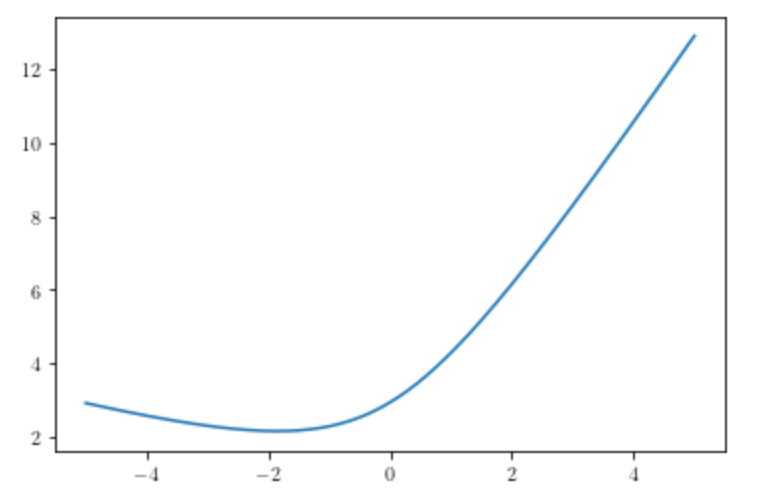
\includegraphics[scale=0.5]{onde_choc.png}
\end{figure}	
	
	\item[$\diamond$] Si $\dif t'/\dif t=0$, alors $t'=t_0$, c'est-à-dire que quelque soit le temps $t$ durant lequel a été émis un son, celui-ci arrivera à l'observateur à $t_0$. Si l'avion émet des sons durant tout son vol (le bruit du réacteur par exemple), tous ces sons arrivent en même temps à $t_0$. Les ondes sonores se supperposent et la puissance reçue est maximale en un instant très court. Il y a un bang !
	
	\item[$\diamond$] $t'_0$ correspond au moment où le bang est perçu par l'observateur, donc d'après la question précédente, correspond au moment où $f'(t_0)=0$.
	\begin{equation}
		f'(t)=1+\frac{v^2t/c^2}{\sqrt{h^2/c^2+v^2t^2/c^2}}
	\end{equation}
	En résolvant l'équation, on trouve que :
	\begin{align*}
		t_0=-\frac{h}{v}\frac{1}{\sqrt{v^2/c^2-1}}
	\end{align*}
	Et :
	\begin{align*}
		t'_0=h\sqrt{1/c^2-1/v^2}
	\end{align*}
	Les positions de l'avion sont $x_0=-h\frac{1}{\sqrt{v^2/c^2-1}}$ et $x'_0=h\sqrt{v^2/c^2-1}$
	
	\item[$\diamond$] L'observateur entend l'avion une fois qu'il se trouve dans le cône dans lequel les ondes sonores sont émises. Il n'entend donc pas l'avion tant qu'il n'a pas entendu le bang. Les sons perçus entre $t'_0$ et $t'_0+\Delta t'$ ont été émis entre $t_0$ et $t_0+\Delta t$. DOnc :
	\begin{align*}
		t'_0+\Delta t'=f(t_0+\Delta t)=f(t_0)+f'(t_0)\Delta t+\frac{1}{2}f''(t_0)\Delta t^2=t'_0+\frac{1}{2}f''(t_0)\Delta t^2
	\end{align*}
	Donc : 
	\begin{align*}
		\Delta t=\sqrt{\frac{2\Delta t'}{f''(t_0)}}, \quad f''(t_0)=\frac{v^2h^2}{c^4(\frac{h^2}{c^2}+\frac{h^2}{v^2-c^2})^{3/2}}
	\end{align*}
	On trouve $\Delta t=0,83$s, cad que le son a bien été compressé (le son perçu est 8 fois plus court). 
	
	\item[$\diamond$] La région atteinte par l'onde sonore émise par l'avion à un instant donné est l'intérieur d'un cône d'angle au sommet $2\theta$ et de sommet le nez de l'avion. 
	
	\item[$\diamond$] L'enveloppe des ondes sonores émises au cours du temps est un cône tangent aux surfaces d'ondes sphériques marquant l'arrivée en un point. On trouve facilement la relation :
	\begin{align*}
		\sin\theta=\frac{c}{v}
	\end{align*}
	Sur la photo, on mesure $\theta\simeq15^\circ$. On a donc $v\simeq352$m.s$^{-1}$. L'avion a juste franchi le mur du son.

\end{itemize}

\section*{Pavillon acoustique}

\begin{itemize}

\item[$\diamondsuit$] Approximation acoustique : $v\ll c$.

\item[$\diamondsuit$] La compressibilité devient $\chi_s=-\frac{1}{V}\frac{\partial V}{\partial P}=-\frac{1}{p(x,t)}\frac{\Psi(x+dx,t)S(x+dx)-\Psi(x,t)S(x)}{S(x)dx}=-\frac{1}{S(x)p(x,t)}\frac{\partial \Psi(x,t)S(x)}{\partial x}$. On trouve ensuite :
\begin{equation}
	p(x,t) = -\frac{1}{\chi_s}\left(\frac{\partial \Psi}{\partial x}+\Psi(x,t)\frac{\partial }{\partial x}\left[\ln S(x) \right]  \right)
	\label{eq:p}
\end{equation}

\item[$\diamondsuit$] L'équation d'Euler :
\begin{align*}
	\frac{\partial^2\Psi}{\partial t^2}+\frac{1}{\rho_0}\frac{\partial p}{\partial x}=0
\end{align*}
On trouve alors :
\begin{equation}
	\frac{\partial^2\Psi}{\partial t^2}-\frac{1}{\chi_s\rho_0}\frac{\partial^2 \Psi}{\partial x^2}=-\frac{\partial}{\partial x}\left(\Psi \frac{\partial \ln S(x)}{\partial x} \right) 
	\label{eq:psi}
\end{equation}

\item[$\diamondsuit$] Pour trouver la même relation sur la pression, on commence par revenir à l'équation $p(x,t) = -\frac{1}{\chi_s}\left(\frac{\partial \Psi}{\partial x}+\Psi(x,t)\frac{\partial }{\partial x}\left[\ln S(x) \right]  \right)$, en la dérivant par rapport à $\partial^2/\partial t^2$ et en utilisant \ref{eq:p} :
\begin{align*}
	\chi_s\rho_0\frac{\partial^2p}{\partial t^2}=-\frac{1}{\chi_s}\left[ \frac{\partial^3 \Psi}{\partial x^3}+2a\frac{\partial^2 \Psi}{\partial x^2}+a^2\frac{\partial \Psi}{\partial x}\right]
\end{align*}
De la même manière, en calculant le terme $\frac{\partial}{\partial x}\left(p \frac{\partial \ln S(x)}{\partial x} \right)$, et en utilisant \ref{eq:psi}, on trouve :

\begin{align*}
	\frac{\partial}{\partial x}\left(p \frac{\partial \ln S(x)}{\partial x} \right) = \frac{\partial^2 p}{\partial x^2}+m\frac{\partial p}{\partial x}=-\frac{1}{\chi_s}\left[ \frac{\partial^3 \Psi}{\partial x^3}+2a\frac{\partial^2 \Psi}{\partial x^2}+a^2\frac{\partial \Psi}{\partial x}\right]
\end{align*}

On a trouve donc  la même relation que \ref{eq:psi} sur la pression.

\item[$\diamondsuit$] On fait un bilan de masse entre $x$ et $x+dx$ (la variation entre ce qu'il y a après et avant est égal à ce qui rentre moins ce qui sort) :
	\begin{align*}
		\rho(x,t+dt)S(x)\dif x-\rho(x,t)S(x)\dif x=\rho(x,t)v(x,t\dif dt)S(x)-\rho(x+dx,t)v(x+dx,t)S(x+dx)
	\end{align*}
où $\rho(x,t)=\mu(x,t)+\rho_0$. Ce qui devient, avec l'approximation acoustique :
	\begin{align*}
		\frac{\partial \mu}{\partial t}S(x)=\rho_0\frac{\partial}{\partial x}\left[ v(x,t)S(x)\right] 
	\end{align*}
	On a alors : 
	\begin{align*}
		\frac{\partial \mu}{\partial t} = -\rho_0\left(\frac{\partial v}{\partial x}+v(x,t)\frac{\partial }		{\partial x}\left[\ln S(x) \right]  \right)
	\end{align*}

\item[$\diamondsuit$]  On injecte la solution proposée dans l'équation. On remarque ce sont des OPPM mais que l'équation n'est pas une équation d'Alembert, mais qui ne tente rien n'a rien. On trouve :
	\begin{align*}
		k^2+jka-\frac{\omega^2}{c^2}=0
	\end{align*}
	Alors, le discriminant est $\Delta=-a^2+4\omega^2/c^2$ :
	\begin{align*}
		k=\frac{1}{2}\left(-j\omega\pm\sqrt{4\frac{\omega^2}{c^2}-a^2}\right) 
	\end{align*}

	Si $4\omega^2/c^2<a^2$ alors $k$ est imaginaire pur, et l'onde ne peut pas se propager, cad si $\omega<\omega_c=ac/2$ :
	\begin{align*}
		p(x,t)=p_0\exp(-kx)\exp(j\omega t)
	\end{align*}
	C'est une onde stationnaire, qui ne se propage pas.
	
	\item[$\diamondsuit$] Si $4\omega^2/c^2>a^2$ :
	\begin{align*}
		p(x,t)=p_0\exp\left(-\frac{ax}{2} \right) \exp\left[ j\left(\omega t- x\frac{\omega}{c}\sqrt{1-\frac{\omega_c^2}{\omega^2}}\right) \right] 
	\end{align*}
	On remarque qu'il y a bien atténuation exponentielle de l'onde : c'est normal, la surface croit exponentiellement et il n'y a pas d'apport d'énergie extérieur. Il y a donc "dilution" exponentielle de l'onde. On remarque que pour des ondes se propageant en sens inverse, l'amplitude augmente exponentiellement (cf utilité de l'oreille).
	
	La vitesse de phase est :
	\begin{align*}
		v_\varphi = \frac{\omega}{\Re\left[ k\right] }=\frac{c}{\sqrt{1-\frac{\omega_c^2}{\omega^2}}}
	\end{align*}
	
	La vitesse de groupe est :
	\begin{align*}
		v_g = \frac{\partial\omega}{\partial \Re\left[ k\right] }=c\sqrt{1-\frac{\omega_c^2}{\omega^2}}
	\end{align*}
	On remarque que $c^2=v_\varphi v_g$.
	
	L'équation d'Euler est :
	\begin{align*}
	\frac{\partial v}{\partial t}+\frac{1}{\rho_0}\frac{\partial p}{\partial x}=0
	\end{align*}
	On a alors :
	\begin{align*}
		v(x,t)=\frac{p_0}{\rho_0\omega}\left[-j\frac{a}{2} +\frac{\omega}{c}\sqrt{1-\frac{\omega_c^2}{\omega^2}}\right] \exp\left(-\frac{ax}{2} \right) \exp\left[ j\left(\omega t- x\frac{\omega}{c}\sqrt{1-\frac{\omega_c^2}{\omega^2}}\right) \right] 
	\end{align*}
	En notation réelle :
	\begin{align*}
		v(x,t)=\frac{p_0}{\rho_0\omega}\exp\left(-\frac{ax}{2} \right)\left[\frac{a}{2}\sin(\omega t-k'x) +k'\cos(\omega t- k'x)\right] 
	\end{align*}	
	Avec $k'=\frac{\omega}{c}\sqrt{1-\frac{\omega_c^2}{\omega^2}}$.
	
	Le vecteur de Poynting s'écrit (en notation réelle !) :
	\begin{align*}
		\vec{\Pi}(x,t)=\left\langle p\vec{v} \right\rangle =k'\frac{p_0^2}{2\rho_0\omega}\exp\left[-\frac{2x}{\delta} \right] 
	\end{align*}
	
	L'énergie acoustique elle s'écrit :
	\begin{align*}
		\varepsilon=\left\langle \frac{\chi_s}{2}p^2+\frac{\rho_0}{2}v^2\right\rangle = \frac{\chi_sp_0^2}{2}\exp\left[-\frac{2x}{\delta} \right] 
	\end{align*}
	Les énergies cinétiques et potentielles sont égales.

\end{itemize}

\subsubsection*{Échographie}

\begin{itemize}
	
	\item[$\spadesuit$] \item[$\circ$] On retrouve l'équation d'Alembert à partir de trois équation. Sur la masse volumique et la compressibilité :
	\begin{align*}
		\mu = \chi_sp\rho_0
	\end{align*}
	Sur l'équation de la conservation de la masse :
	\begin{align*}
		\frac{\partial \mu}{\partial t}+\grad(p)=0
	\end{align*}
	et l'équation d'Euler :
	\begin{equation}
		\rho_0\frac{\partial \vec{v}}{\partial t}+\vec{\grad}(\vec{v})=0
	\end{equation}
	On trouve alors une équation d'Alembert sur $\mu$, $\vec{v}$ et $p$, avec une célérité $c=1/\sqrt{\chi_s\rho_0}$.
	 Les solutions générales sont sous la forme $p(x,t)=f(t-x/v) + g(t+x/v)$, représentant une onde se propageant selon les $x$ croissants et décroissants.
	
	\item[$\spadesuit$] On trouve avec l'équation d'Alembert 
	\begin{align*}
		k_j=\pm\omega/c_j
	\end{align*}
	Avec les équation différentielles couplées entre $\vec{v}$ et $p$ on a :
	\begin{align*}
		p_j=\pm\rho_j c_j v_j = Z_jv_j
	\end{align*}
	Le signe $\pm$ est positif si l'onde se propage selon les $x$ croissant, négatif dans les cas contraire. $Z_j$ est l'impédance acoustique du milieu $j$.
	
	\item[$\spadesuit$] Avec respectivement la conservation du débit et le principe fondamental de la dynamique, on a en $x=0$ :
	\begin{align*}
		\vec{v}_1(0,t)&=\vec{v}_2(0,t) \\
		p_1(0,t)&=p_2(0,t)
	\end{align*}
	
	\item[$\spadesuit$] S'il n'y avait pas d'onde réfléchie (cad d'onde se propageant vers les $x$ décroissant dans le milieu 1), on aurait avec les deux expressions précédentes :
	\begin{align*}
		v_{0,1}&=v_{0,2} \\
		v_{0,1}Z_1&=v_{0,2}Z_2
	\end{align*}
	Comme $Z_1\neq Z_2$, on aurait $v_{0,1}=v_{0,2}=0$, c'est à dire rien. Il y a nécéssairement une onde réfléchie, cad :
	\begin{align*}
		v_1(x,t)&=v_{0,i}\exp\left[i(k_1x- \omega t) \right]+v_{0,r}\exp\left[i(k_1x+ \omega t) \right]\\
		v_2(x,t)&=v_{0,t}\exp\left[i(k_1x- \omega t) \right]
	\end{align*}
	
	\item[$\spadesuit$] Avec les relations de continuité, on trouve :
	\begin{align*}
	r_v&=\frac{Z_1-Z_2}{Z_1+Z_2}\\
	t_v&=\frac{2Z_1}{Z_1+Z_2}
	\end{align*}
	et (pour la pression, les relations de continuité reviennent à remplacer $r_v\leftarrow r_p$, $t_v\leftarrow t_p$ et $Z_j\leftarrow 1/Z_j$ :
	\begin{align*}
	r_p&=\frac{Z_2-Z_1}{Z_1+Z_2}\\
	t_p&=\frac{2Z_2}{Z_1+Z_2}
	\end{align*}
	
\item[$\spadesuit$] Pour une OPPM, on a les relations énergétiques suivantes :
	\begin{align*}
		\left\langle \vec{R_s} \right\rangle &=\frac{1}{2}\rho v_{0}^2 c \vec{e}_x \\
		\left\langle \varepsilon \right\rangle &= \frac{1}{2}\rho v_{0}^2
	\end{align*}	
	où $\vec{R_s}$ est le vecteur d'intensité sonore et $\varepsilon$ l'énergie volumique de l'onde sonore. 
	L'intensité sonore est simplement $I_s = \|\vec{R_s} \|$. On a alors :
	\begin{align*}
		I_{S,i}&=\frac{1}{2}\rho_1 c_1 v_{0,i}^2 \\
		I_{S,r}&=\frac{1}{2}\rho_1 c_1 v_{0,r}^2 \\
		I_{S,t}&=\frac{1}{2}\rho_2 c_2 v_{0,t}^2 
	\end{align*}
	On a alors :
	\begin{align*}
		R =& \frac{ v_{0,i}^2}{ v_{0,r}^2}=r_v^2=\left( \frac{Z_1-Z_2}{Z_1+Z_2}\right) ^2\\
		T &= \frac{Z_2}{Z_1}t_v^2=\frac{4Z_1Z_2}{Z_1+Z_2}^2
	\end{align*}		
	
	\item[$\spadesuit$] Pour un écho, on souhaite transmettre des ondes sonores entre une sonde solide et le corps humain (liquide) qui ont des impédances très élevées. Si une couche d'air se glisse entre la sonde et le corps, l'impédance de l'air étant très faible par rapport à celle de la sonde ($Z_1\gg Z2$), les coefficients de transmission en énergie sont :
	\begin{align*}
		R \gg T
	\end{align*}
	Il n'y a pas ou très peu d'onde sonore qui arrive dans le corps humain.
		
\end{itemize}

\subsubsection*{Isolation phonique}

On suppose qu'il y a désormais une paroi de masse surfacique $\mu$ à l'interface entre les deux milieux, qui sont supposées être identiques ($\rho_1=\rho_2$ et $c_1=c_2$). Cette paroi se meut librement et sans frottement. 

\begin{itemize}
	
	\item[$\clubsuit$] On a toujours la continuité de la vitesse, due à la conservation du débit :
	\begin{align*}
		v_{0,i}+v_{0,r}=v_{0,t}
	\end{align*}
	Pour le PFD, c'est différent à cause du mur, où sa vitesse est supposée être $V$ (qui est nécessairement égale à celle de l'onde transmisse :$V=v_{0,t}$par continuité de la vitesse) :
	\begin{align*}
		\mu S\frac{dV}{dt}=S(p_1-p_2)=S(p_{0,i}+p_{0,r}-p_{0,t})
	\end{align*}
	En remplaçant avec les impédances respectives, on obitent :
	\begin{align*}
		j\omega\mu v_{0,t}=Z_1(v_{0,i}-v_{0,r})+Z_2v_{0,t}
	\end{align*}
	On trouve alors si les deux milieux sont identiques ($Z_1=Z_2=Z$) :
	\begin{align*}
		t_v= \frac{v_{0,t}}{v_{0,i}}= \frac{1}{1+i\omega\frac{\mu}{2Z}}
	\end{align*}
	
	\item[$\clubsuit$] On trouve :
	\begin{align*}
		T= |t|^2=\frac{Z_1|v_{0,t}|^2}{Z_2|v_{0,i}|^2}=|t_v|^2=\frac{1}{1+\omega^2\tau^2}
	\end{align*}
	avec $\tau=\mu/2Z$. C'est un passe-bas d'ordre 1 avec une pulsation de coupure $\omega_c=1/\tau$.
	
	\item[$\clubsuit$] De combien doit être l'épaisseur d'un mur de béton entre deux logements d'un appartement pour que l'atténuation soit atténuée de 50dB à 300Hz ? On donne $\rho_{béton}=2300$kg.m$^{-3}$. 
	En décibel, on a $20\log$ 
	
\end{itemize}


\end{document}
